\mychapter{4}{MultiVariate Analysis}
\label{sec:unchapitre}

Now that we get background and signal samples we can perform the MVA for classification.\\
For this purpose the TMVA framework from ROOT was used. Multiple MVA techniques were tested fig. (\ref{mva_multiple}) with default configuration then the 2
bests were selected for the tuning of their parameters : the ANN and BDT\\

\begin{figure}[h!]
\centering
    \begin{subfigure}[h!]{0.4\textwidth}
    \centering
        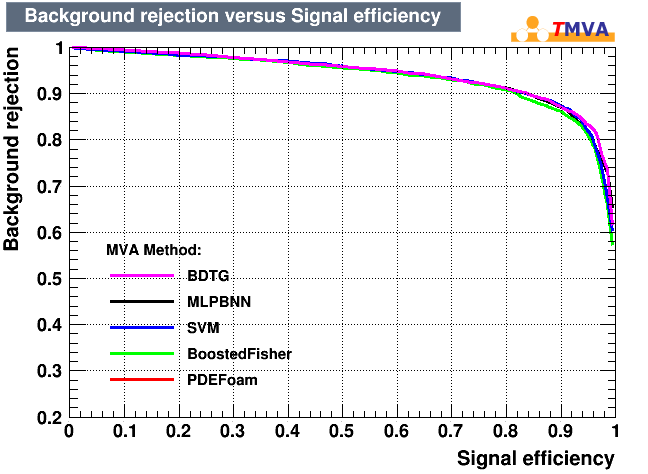
\includegraphics[width=\textwidth]{mva_multiple}
        \caption{ROC curves of 5 bests MVA, these are almost overlapping.}
        \label{mva_multiple}
  \end{subfigure}
  ~
    \begin{subfigure}[h!]{0.4\textwidth}
    \centering
        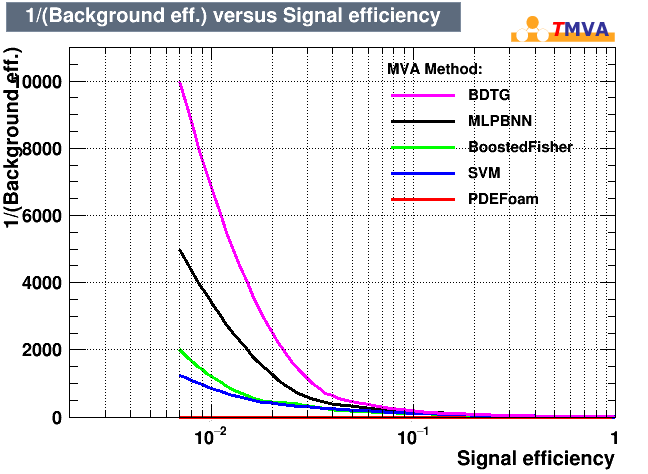
\includegraphics[width=\textwidth]{inv_mva_multiple.png}
        \caption{Inverse ROC curve for the 5 bests MVA, on this plot BDT and ANN(MLPBNN) are clearly the two bests.}
        \label{inv_mva_multiple}
  \end{subfigure}
  \caption{ROC curve for the 5 best MVA that has been tested. Receiver Operating Characteristic (ROC) curve reflects the discrimination power of a classifier. It is constructed by plotting the ratio of background rejection versus signal efficiency by varying a threshold on the MVA output.}
\end{figure}


\section{Artificial Neural Network}

An ANN is a multilayer perceptron with fully interconnected layers fig. (\ref{nn_arch}).
This ANN is used for classification, it is a function mapping an input vector $\vec{x_0}$ (input variables) to a scalar
$y$ with $y \in [0;1]$ (classification category).\\
Fig. (\ref{nn_output}) shows the output $y$ of the ANN that has been trained. Data have been divided in two, one
training sample and one testing sample.

%\subsection{Theory}

A neuron is referenced by his position in the network, a neuron $h_{i,j}(\vec{x_{j-1}}) \rightarrow h_{i,j}$ represent the i-th neuron of the j-th layer.\\
Such neuron sums all neuron's output in the (j-1)-th layer, weighted by their connection weight. This net sum is then evaluated through the activation function ( sigmoid, logistic, heaviside, linear, etc) fig. (\ref{one_neuron}).

\begin{figure}[h!]
\centering
    \begin{subfigure}[h!]{0.6\textwidth}
    \centering
    	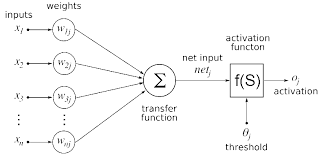
\includegraphics[width=\textwidth]{one_neuron}
    	\caption{Diagram of a single neuron algorithm.}
    	\label{one_neuron}
	\end{subfigure}
	~
    \begin{subfigure}[h!]{0.35\textwidth}
    \centering
    	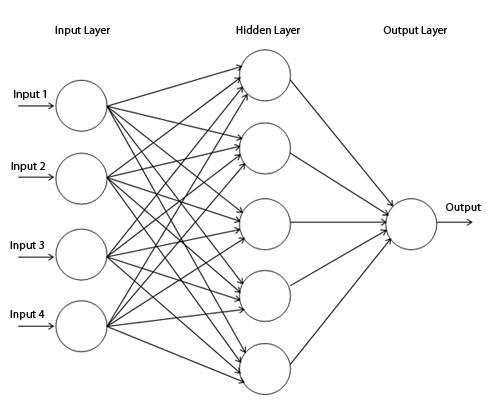
\includegraphics[width=\textwidth]{nn_arch}
    	\caption{Architecture of an artificial neural network with 4 input variables, one hidden layer, and one output neuron.}
    	\label{nn_arch}
	\end{subfigure}
\end{figure}


A lot of parameters are available for tuning :
\begin{description}
    \item [Input variables] Choice of input variable set, number of variables, choice of a Pre-processing method, etc.
    \item [ANN architecture] number of hidden layers, number of neurons per layer, choice of an activation function, etc.
    \item [Learning algorithm parameter] Choice of a learning method, choice of a regulator, value of learning rate, step size, weight decay rate, etc.
\end{description}

All of these cannot be optimize at the same time, so a choice has to be made.\\
The first parameter to be tune is the input variable set, a compromise has to be made in order to have the smallest input set but containing the most relevant information for classification.

\subsection{Input set optimization}

For this part an iterative process of optimization will be performed :
\begin{description}
	\item [step 1] Train MVA with full input variable set
	\item [step 2] Train N MVA removing one variable at a time
	\begin{description}
		\item [step 2.1] The MVA that succeed the best despite of having removed one variable, tells us that this variable wasn't revelant.
		\item [step 2.2] Remove this variable permanently, reiterate step 2 until no variable is left.
	\end{description}
	\item [final step] keep the input variable set of the best MVA
\end{description}

For evaluating the ANN multiple estimators has been tested :
\begin{description}
	\item [Mean Square Estimator (MSE)] $ MSE(\hat{\theta}) = E_{\hat{\theta}} [(\hat{\theta} - \theta)^2] =
    Var_{\hat{\theta}} + Bias(\hat{\theta}, \theta)^2$
	\item [Cross-Entropy (CE)] $ H(T,q) = -\sum_{i=1}^{N}{\frac{1}{N} log_2 q(x_i)}$
	\item [Overlapping criteria] is the sum of the products of signal and background response in each bin $ OC =
    \sum_{i=1}^{N}{signal_i*background_i} $ with $N :=$ number of bins , $signal_i := $ number of signal events in bin
    number i $background_i := $ number of background events in bin number i. Good classifiers show low value for this estimator.
\end{description}

\begin{figure}[h!]
\centering
    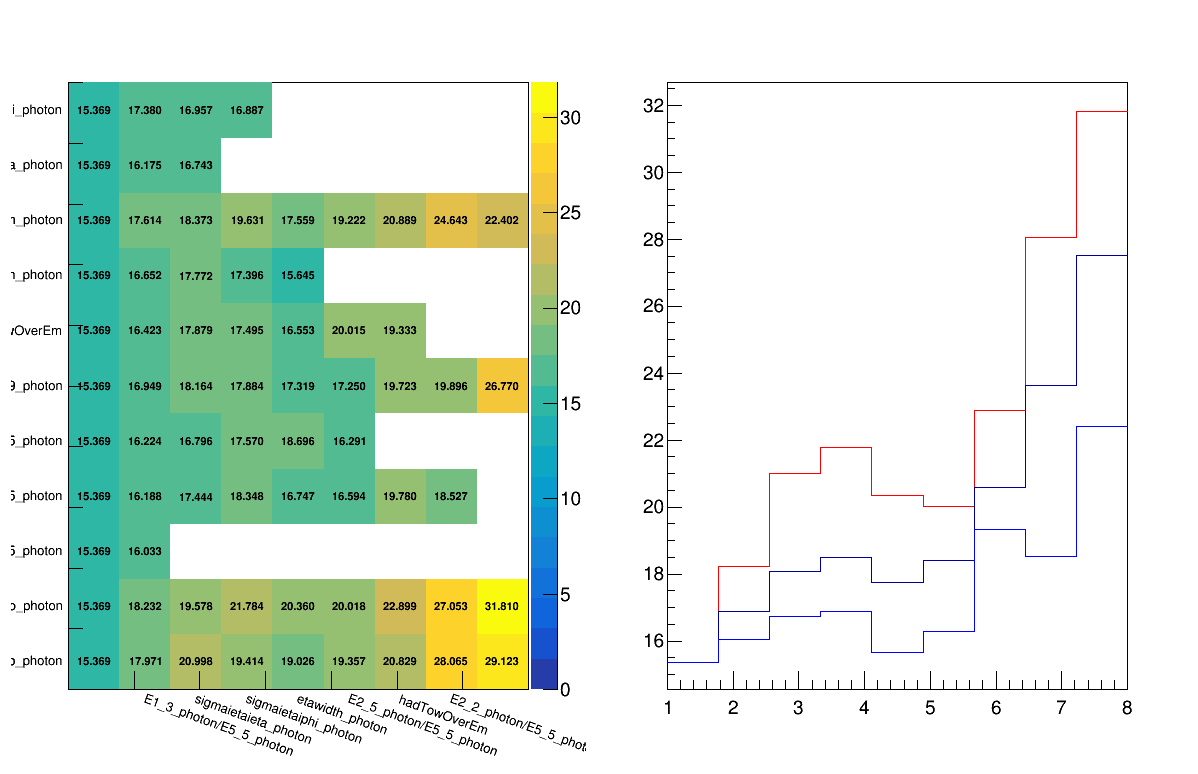
\includegraphics[width=1.\textwidth]{input_optim}
    \caption{On the left : Input variable set optimization results overview for the "overlapping criteria" estimator.
    Each bin is the estimator value for one MVA. Except for
    the 1st column that represents the MVA trained with the whole input seti (step 1), 2nd column
    represent MVA's that has been trained after removing one variable at a time (step 2), following columns are the
    iterations of step 2.\\
    On the right : overview of the estimator value for each column (step 2). maximum value (red solid line), average
    value (dark blue solid line) and lowest value (light blue solid line).}
    \label{input_optim}
\end{figure}

The optimization results in fig. (\ref{input_optim}) shows that keeping all the variables lead to the best MVA. So the whole input set will be used for the training. The ANN fig. (\ref{nn_output}) used 11 input variables : neutral hadron isolation, photon isolation, $\sigma_{i \eta i \eta}$, $\sigma_{i \eta i \phi}$, $\eta_{width}$, $\phi_{width}$, $R_9$, Had/Em, $E_{1x3}/E_{5x5}$, $E_{2x2}/E_{5x5}$ and $E_{2x5}/E_{5x5}$.
 
\begin{figure}[h!]
\centering
    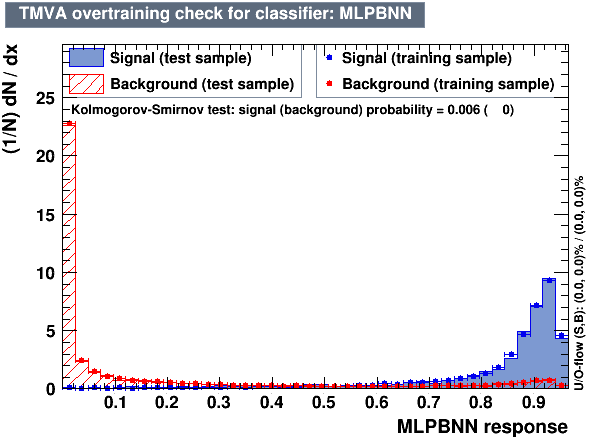
\includegraphics[width=0.6\textwidth]{nn_output}
    \caption{Artificial Neural Network response with signal from test sample (blue histogram), background from test
    sample (red shaded histogram), signal from training sample (blue dots) and background from training sample (red
    dots). The good agreement between training and testing sample shows no overfitting (in the case where these sample
    are representative of the data).}
    \label{nn_output}
\end{figure}

\section{Boosted Decision Tree}

Being the best MVA method a BDT has been trained also for the next part of the analysis fig. (\ref{bdt_output}).
Multiple learning method has been used, the Gradient Boost Method was the most efficient one.
\begin{figure}[h!]
\centering
    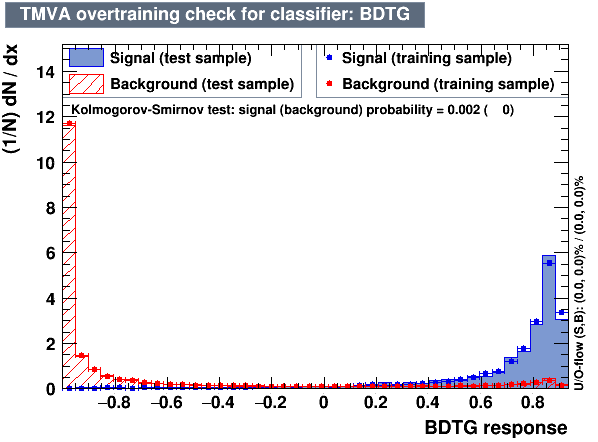
\includegraphics[width=0.6\textwidth]{bdt_output}
    \caption{Boosted Decision Tree response.}
    \label{bdt_output}
\end{figure}

%\subsection{Theory}

BDT uses a decision tree in order to map from input variables to the event category (signal or background).
For this kind of classification tree, branches represent relations between variable or cuts on variables that lead to leaf representing category of the event.\\
For the "Gradient Boosting" method, the classification is done by combining together weak classifiers in an iteratively way.
A finir!!!

%%% Local Variables: 
%%% mode: latex
%%% TeX-master: "isae-report-template"
%%% End: 

